\chapter{文明、科学与AI：自反结构演化}

\begin{chapteroverviewbox}
本章处于全书第一编“认识论”的收束位置。此前我们已经从智能的时空尺度、多频闭环、CSO 与 Agent-CSO、功能拓扑、结构迁移以及 World--Agent--World 双向闭环出发，得到一个关键结论：智能并不是宇宙之外的观察者，而是宇宙内部出现的一类能够形成关于其他结构以及自身结构的内部表示，并使这些表示参与未来现实变化的特殊结构。

本章进一步讨论，当这种能力不再局限于单个 Agent，而通过语言、文字、制度、科学、技术和人工智能跨主体、跨生命周期积累之后，会发生怎样的尺度跃迁。我们将文明理解为一种由大量个体、外部记忆、制度、工具、技术系统和公共认知结构共同构成的慢尺度适应系统；将科学理解为文明尺度上持续校准世界模型的机制；将工程理解为把内部表征重新投射到现实的主动修改机制；将社会制度理解为历史性 CSO 流沉降形成的功能拓扑；并将 AI 的出现解释为文明外部认知结构从“被动存储”向“主动表征、推理、预测和控制”迁移的重要阶段。

这里必须严格保持理论边界。本章所谓“文明的自我观察”“宇宙通过文明认识自身”“文明尺度 SPC/TCE”等表述，均属于\textbf{结构动力学和功能同构意义上的理论描述}，并不意味着我们已经证明文明具有单一主体意识，也不意味着宇宙整体具有目的、意志或现象意识。已有科学能够支持的是语言、文化传播、外部记忆、集体认知、科学建模、技术反馈和人工智能等具体过程；而将这些过程统一为“自反结构演化”（Reflexive Structural Evolution），属于本书在这些事实之上提出的更高层理论框架。

本章最终要建立的核心命题是：
\begin{statementbox}
文明的发展，本质上不断提高现实结构形成关于自身的公共表示、
预测自身未来并依据这些表示重新组织现实的能力。
\end{statementbox}

而人工智能的重要历史意义，则可能表现为这种闭环在表示带宽、整合尺度、预测深度、控制速度和自我重组能力上的进一步跃迁。
\end{chapteroverviewbox}

\begin{figure}[htbp]
\centering
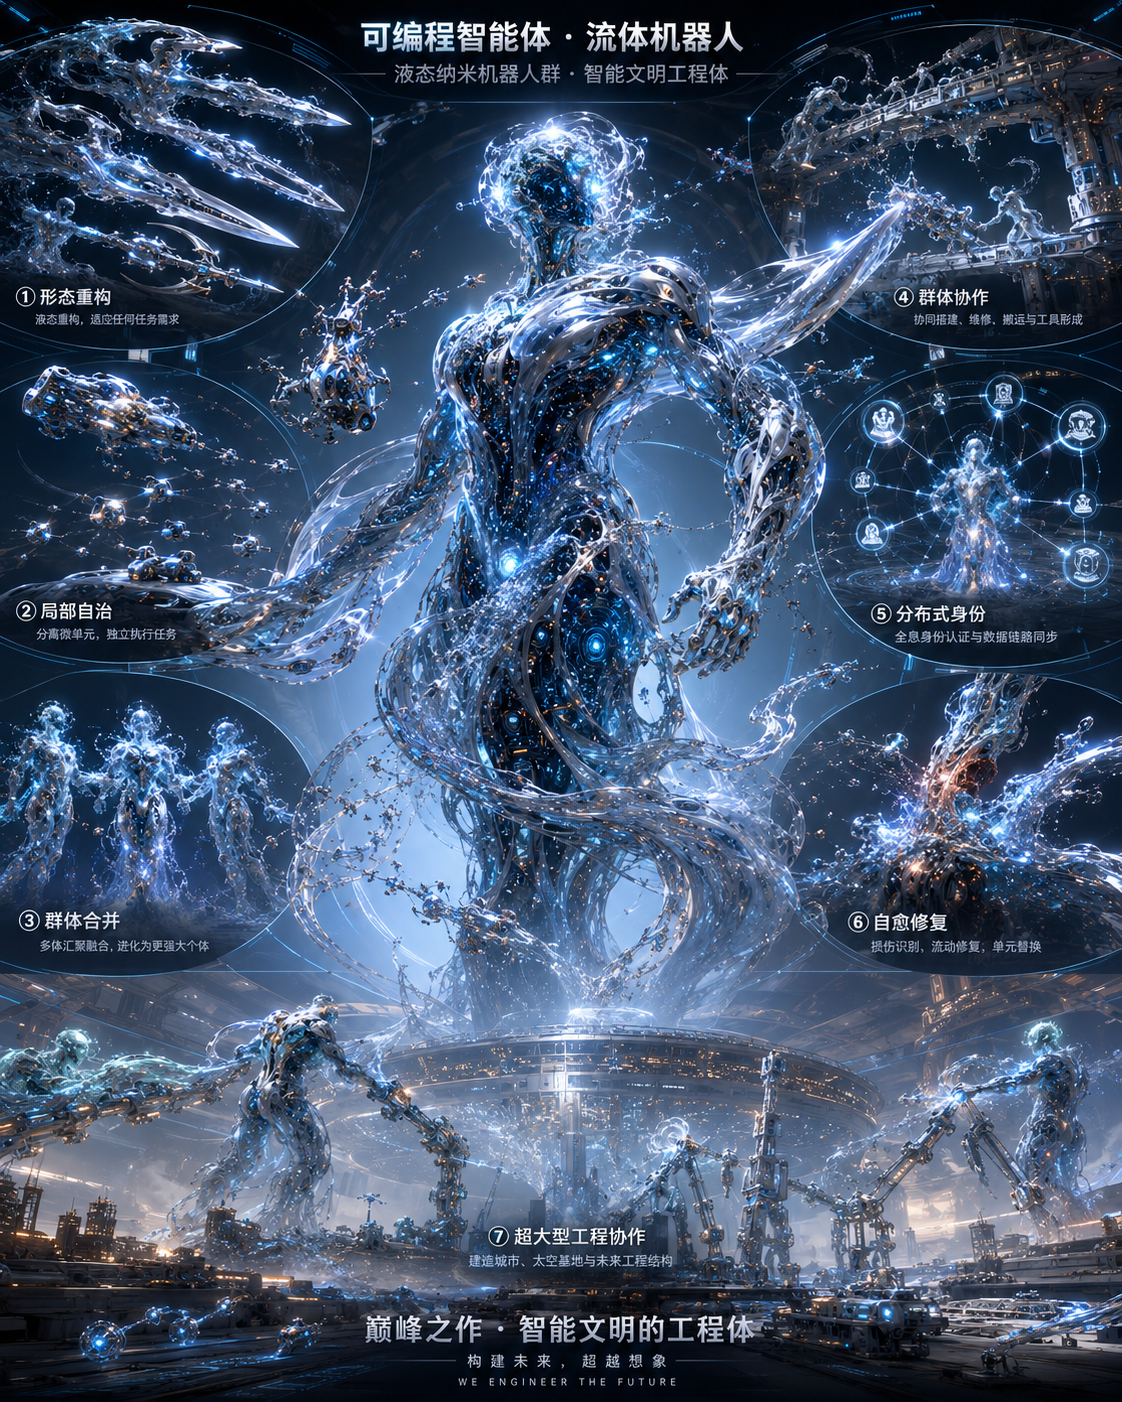
\includegraphics[width=.9\textwidth,height=.38\textheight,keepaspectratio]{images/cognitive-cosmos-artwork.png}
\caption{语言、科学、工程与文明自反闭环}
\end{figure}
\section{语言：Agent-CSO 的跨主体共享接口}

在前面的讨论中，我们已经把单个智能体所拥有的内部认知结构定义为 Agent-CSO。一个外部现实结构 $C$ 经过智能体 $A$ 的观察、选择、压缩和内部建模之后，并不会以现实本身的形式直接存在于智能体内部，而是形成该智能体特有的结构实现：
\[
\pi_A:C\rightarrow C_A ,
\]
其中 $C_A=\pi_A(C)$ 是 Agent $A$ 对本体结构 $C$ 的具体承载。由此产生一个根本问题：如果每个 Agent-CSO 都被封闭在一个具体主体内部，那么智能即使能够在个体生命周期中积累，也很难形成真正跨主体的结构成长。个体死亡、失忆或环境改变，都可能使已经形成的大量认知结构重新消失。

语言的出现改变了这一局面。我们可以把语言理解成一种把内部 Agent-CSO 投影到公共符号空间中的结构映射。设智能体 $A$ 的内部结构为 $C_A$，语言编码函数为
\[
L_A:C_A\rightarrow s,
\]
其中 $s$ 是能够进入公共环境的语言符号结构。另一个智能体 $B$ 接收到 $s$ 后，通过自己的解释映射
\[
D_B:s\rightarrow \hat{C}_B
\]
形成自身内部的近似结构。于是完整过程为
\[
C_A
\xrightarrow{L_A}
s
\xrightarrow{D_B}
\hat{C}_B.
\]

这里需要特别注意：
\[
\hat{C}_B\neq C_A
\]
通常才是正常情况。语言从来不是把一个人的内部状态逐比特复制到另一个人的大脑，而是在两个不同认知系统之间建立结构约束，使二者能够形成足够相似、足以协作的认知结构。因此，语言真正完成的不是 ``state copying''，而是
\begin{statementbox}
Structural Coordination
\end{statementbox}
即结构协调。

如果存在一个本体 CSO $C$，两个主体分别形成
\[
C_A=\pi_A(C),\qquad
C_B=\pi_B(C),
\]
那么语言的作用不是强制满足
\[
C_A=C_B,
\]
而是在任务相关关系上降低两者的结构差异。可以概念性地定义一个语义等价度：
\[
\Sigma(C_A,C_B)
=
F(
R_{\mathrm{semantic}},
R_{\mathrm{causal}},
R_{\mathrm{functional}},
R_{\mathrm{predictive}}
),
\]
其中分别衡量语义关系、因果关系、功能关系和预测关系的保持程度。当
\[
\Sigma(C_A,C_B)>\theta_{\mathrm{communication}},
\]
两个 Agent 即使拥有不同的内部表示，也已经能够围绕该 CSO 形成有效协作。

从这一角度看，语言第一次大规模打开了智能体的认知边界。此前的结构循环主要是
\[
World
\rightarrow
Agent_A
\rightarrow
World,
\]
语言出现以后，世界中开始出现
\[
Agent_A
\rightarrow
Symbol
\rightarrow
Agent_B
\]
的跨主体认知路径。一个主体通过自身生命史形成的结构，可以成为另一个主体形成 Agent-CSO 的输入。因此，社会中的认知结构不再必须由每个人从现实中独立重新发现。

我们可以把这种结构收益写成
\[
C_{\mathrm{social}}
\neq
\sum_i C_i
\]
的简单累加，而更接近
\[
\mathcal{G}_{\mathrm{social}}
=
\left(
\bigcup_i \mathcal{G}_{C}^{(i)},
E_{\mathrm{language}}
\right),
\]
其中 $\mathcal{G}_{C}^{(i)}$ 是第 $i$ 个个体的认知结构图，而 $E_{\mathrm{language}}$ 是通过语言建立的跨主体结构耦合关系。语言因而使原本相互隔离的局部 Agent-CSO 图首次能够形成更大的公共认知网络。

这里与外部已有理论存在明显联系。分布式认知理论强调认知过程可以跨越单个大脑而分布于主体、符号和环境之间；语言学、符号学和社会认知理论研究符号如何使不同主体协调意义；信息论则能够分析通信带宽和噪声。然而，本书进一步强调的不是“信息从一个节点传到另一个节点”，而是\textbf{CSO 的跨主体重新实现}。语言的根本作用不只是提高信息流量，而是使
\[
AgentCSO_A
\rightarrow
ExternalCSO
\rightarrow
AgentCSO_B
\]
成为稳定可重复的结构过程。

正是在这个意义上，我们可以把语言称为文明形成以前最关键的第一类“认知 ABI”。它第一次提供了一种与具体神经实现相对独立的公共接口，使结构可以脱离原始载体，以符号形式跨越主体边界重新获得承载。这为文字、制度、科学乃至人工智能的产生奠定了共同基础。


\section{文字：跨生命周期的结构记忆}

语言解决的主要是跨主体结构传播问题，但口语本身仍然高度依赖主体的同时存在。如果说语言主要建立
\[
Agent_A(t)
\leftrightarrow
Agent_B(t)
\]
的同步耦合，那么文字真正改变的是时间维度：
\[
Agent_A(t_0)
\rightarrow
Agent_B(t_1),
\qquad
t_1\gg t_0.
\]

这意味着 Agent-CSO 第一次能够系统地脱离原主体的生理生命周期，在更长时间尺度上继续存在。设某个主体在 $t_0$ 时刻拥有结构
\[
C_A(t_0),
\]
经过外化编码成为
\[
C_{\mathrm{ext}}
=
W\left(C_A(t_0)\right).
\]
只要外部介质继续存在，另一个未来主体 $B$ 就可以在 $t_1$ 时刻执行
\[
C_B(t_1)
=
R_B(C_{\mathrm{ext}}),
\]
其中 $R_B$ 表示阅读、解释和重新建模过程。

于是知识不再严格受到
\[
\tau_{\mathrm{knowledge}}
\leq
\tau_{\mathrm{individual}}
\]
这一限制，而可以出现
\[
\tau_{\mathrm{external\ structure}}
\gg
\tau_{\mathrm{individual}}.
\]

这是一种非常重要的时间尺度跃迁。

在三相记忆理论中，我们曾经把个体内部的 $E$ 理解为经验轨迹，把 $\Theta$ 理解为较慢的结构性生成记忆。如果把尺度扩大到文明，我们会发现文字和其他持久化媒介承担了一种类似外部长期结构记忆的功能：个体中的经历和结构可以被写入公共环境，成为文明后续 Agent 的可恢复认知资源。

因此，文明记忆不是一个超级大脑中的单一数据库，而是一套分布于
\[
\{\text{文本、档案、图表、仪器、数据库、建筑、法律、程序、标准}\}
\]
中的结构网络。可以定义文明的外部记忆集合
\[
\mathcal{M}_{\mathrm{civil}}
=
\{M_1,M_2,\ldots,M_n\},
\]
并通过访问关系
\[
A_{ij}
\]
描述第 $i$ 类主体对第 $j$ 类外部结构的可恢复能力。于是文明实际可使用的记忆不只是所有存储对象的总和，而取决于
\[
\boxed{
EffectiveMemory
=
StoredStructure
\times
Indexability
\times
Interpretability
\times
Accessibility
}
\]

如果一个结构被保存了，却没有索引；或者有索引，却已经没有主体能够解释，那么它虽然仍然是一个物理 External-CSO，却已经部分失去文明认知记忆的功能。

这一点与我们此前的 Offloading 理论完全一致。认知卸载并不是简单把内部内容“扔到外面”，而要求保留
\[
InternalIndex
\leftrightarrow
ExternalCarrier
\]
的稳定映射。只有当未来系统仍然能够恢复、调用和重新整合外部结构时，外化才真正构成认知能力的扩展。

所以，从更高尺度看，文字可以理解为文明第一次大规模实现
\begin{statementbox}
CognitiveOffloadingAcrossGenerations
\end{statementbox}
即跨代认知卸载。

这一变化又进一步改变了人类社会的学习方式。没有持久化外部记忆时，每一代主体需要重新经历大量世界才能形成结构；文字以后，下一代可以直接从前一代已经形成的高度压缩 Agent-CSO 开始。于是文明发展速度不再只由个体的学习速度决定，而出现
\[
\frac{d\mathcal{K}_{\mathrm{civil}}}{dt}
=
F\!\left(
\begin{gathered}
\mathrm{Discovery},\ \mathrm{Externalization},\ \mathrm{Preservation},\\
\mathrm{Transmission},\ \mathrm{Reinterpretation}
\end{gathered}
\right).
\]

这里 $\mathcal{K}_{\mathrm{civil}}$ 不是一个简单的信息数量，而是文明可实际调用的结构知识集合。

因此，我们可以作出一个很重要的区分：

个体记忆解决的是
\begin{statementbox}
How does this Agent remain itself over time?
\end{statementbox}

文明记忆解决的是
\begin{statementbox}
How can cognitive structure survive the disappearance of its original Agent?
\end{statementbox}

前者形成身份连续性，后者形成文化连续性。

外部已有理论中的文化传播、外部记忆、扩展心智、分布式认知和累积文化理论都与这一讨论有明显关联。本书在此基础上强调：文明真正发生的是 Agent-CSO 的\textbf{载体迁移和生命周期解耦}。结构原来依附于某一个主体，后来被迁移到能够跨越多个主体寿命的外部载体，从而产生比任何个体更慢的文明认知时间尺度。


\section{科学：文明尺度的世界模型校准机制}

语言和文字使认知结构能够传播和保存，但这并不自动保证保存的结构与现实一致。一个社会完全可以长期保存大量错误结构。因此，文明进一步需要一种能够不断把公共 Agent-CSO 与 Universe-CSO 重新比较的机制。科学的独特地位就在这里。

我们可以把一个科学理论抽象成文明内部形成的结构模型
\[
M_\theta,
\]
其中 $\theta$ 表示理论参数、结构关系和假设。给定现实状态 $U_t$，理论产生预测
\[
\hat{Y}_{t+\Delta}
=
P(M_\theta,U_t).
\]
实验或观测随后产生现实结果
\[
Y_{t+\Delta}
=
O(U_{t+\Delta}),
\]
两者之间形成残差
\[
\varepsilon_t
=
D(
Y_{t+\Delta},
\hat{Y}_{t+\Delta}
).
\]

于是科学的基本闭环可以写成
\[
\boxed{
Theory
\rightarrow
Prediction
\rightarrow
Observation/Experiment
\rightarrow
Residual
\rightarrow
TheoryUpdate
}
\]

这与我们此前讨论的 Agent 预测闭环具有明显的结构同构：
\[
Prediction
\rightarrow
Action
\rightarrow
Observation
\rightarrow
Residual
\rightarrow
Update.
\]

但科学系统的重要之处在于，这个闭环不是局限于一个 Agent 的认知过程，而是通过论文、实验协议、同行验证、仪器、数据库和教育体系实现跨主体的长期延续。于是科学可以被理解成一个分布式、超慢速、具有强现实反馈约束的文明模型更新系统。

如果我们使用前面关于 SPC 的一般定义：
\[
SPC:
DistributedState
\rightarrow
AccessibleStateEstimate,
\]
那么从功能同构角度，科学系统确实承担了部分文明尺度的 SPC 功能。它不断回答：

\begin{quote}
世界现在是什么样？\\
我们所处的位置是什么？\\
过去发生了什么？\\
哪些结构关系是稳定的？\\
我们的理论在哪些地方与现实不一致？
\end{quote}

不过必须再次强调：
\[
\boxed{
Science\neq LiteralCivilizationalSPC
}
\]
这里不是声称科学系统就是一个真正的软件 SPC 模块，而是说它在更高尺度上完成了相似的功能任务：把分散的现实观测压缩成可共享、可检验和可进一步使用的结构描述。

这种文明尺度的自观察能力随着历史显著增强。早期社会能够可靠观测的结构范围非常局部；现代文明则通过望远镜、显微镜、粒子探测器、气象卫星、全球定位、基因测序、互联网测量和各种传感器网络扩大了观察函数
\[
O_{\mathrm{civil}}.
\]
因此文明可形成的公共结构集合从
\[
\mathcal{C}_{\mathrm{local}}
\]
逐渐扩展到
\[
\mathcal{C}_{\mathrm{planetary}},
\qquad
\mathcal{C}_{\mathrm{galactic}},
\qquad
\mathcal{C}_{\mathrm{cosmological}},
\qquad
\mathcal{C}_{\mathrm{microscopic}}.
\]

这里发生了两个独立增长：

\[
\boxed{
ObservationCoverage\uparrow
}
\]

和

\[
\boxed{
ObservationResolution\uparrow
}
\]

文明不仅看得更远，也看得更细。

科学的第二个重要性质是结构压缩。一个好的理论并不复制每一次具体观测，而是形成能够解释和预测大量事件的稳定结构：
\[
E_{\mathrm{many}}
\rightarrow
\Theta_{\mathrm{scientific}}.
\]
这一过程与三相记忆中的
\[
E\rightarrow\Theta
\]
具有直接的结构相似性。实验和观测形成大量“文明情景经验”，科学理论则从中抽取更慢、更稳定的生成关系。因此，我们甚至可以把科学进步理解为文明尺度上的经验压缩和结构记忆形成过程。

然而科学系统同样存在认知滞后。文明对现实的模型永远建立在已有观测基础上：
\[
p(
U_t
\mid
O_{\leq t}
),
\]
而不可能完全等于
\[
U_t.
\]
因此科学不是获得“现实本身”，而是在持续现实反馈中形成可修正的 Agent-CSO。科学知识的强大之处不在于它绝对无误，而在于它维持了
\begin{statementbox}
Error-CorrectableRealityCoupling
\end{statementbox}
即一种允许现实不断纠正内部结构的开放闭环。

这也是本书反复强调
\begin{statementbox}
RealityIsUltimateConstraint
\end{statementbox}
的文明尺度版本。


\section{工程：内部结构重新进入现实}

如果科学主要强化文明的
\[
World\rightarrow Representation
\]
路径，那么工程则强化
\[
Representation\rightarrow World
\]
路径。

一个 Agent 形成关于现实的模型以后，并不必然产生智能意义上的现实改变。只有当内部结构通过行动重新进入世界，Agent-CSO 才真正成为外部现实动力学的一部分。因此，工程技术的本质可以从 CSO 理论重新表达为
\[
\boxed{
AgentCSO
\rightarrow
DesignedExternalCSO
}
\]

例如，一个建筑在建成以前首先可能以计划、几何结构、功能要求和约束条件存在于人的内部或外部认知系统中：
\[
C_{\mathrm{building}}^{\mathrm{possible}}.
\]
经过设计、资源组织和现实行动以后，它变成
\[
C_{\mathrm{building}}^{\mathrm{actual}}.
\]
于是发生：
\[
AgentCSO(\mathrm{possible\ world})
\rightarrow
ActionSequence
\rightarrow
UniverseCSO(\mathrm{actual\ world}).
\]

这说明工程引入了一个非常重要的因果形式：
\[
\boxed{
RepresentationOfPossibleFuture
\rightarrow
PresentAction
\rightarrow
ActualFuture
}
\]

这里并不存在真正的“未来反向因果”。真正作用于现在的是一个当前已经物理存在于智能系统中的\textbf{未来表征}。可能未来以 Agent-CSO 的形式进入当前动力学，从而改变实际未来。

这是智能与普通无表征动力过程之间最重要的差异之一。

我们可以进一步定义文明的行动能力
\[
\mathcal{A}_{\mathrm{civil}}
=
\{a_1,a_2,\ldots,a_m\},
\]
以及在世界状态 $U_t$ 下的可达集合
\[
\mathcal{R}(U_t,\mathcal{A}_{\mathrm{civil}})
=
\left\{
U_{t+\Delta}
\,\middle|\,
\exists a\in\mathcal{A}_{\mathrm{civil}}
\right\}.
\]

技术进步的重要含义之一，就是扩大
\begin{statementbox}
ReachableRealitySet
\end{statementbox}
即文明能够通过行动到达的现实状态集合。

火的使用扩展了能量控制范围；农业扩大了生态结构修改范围；机械扩大了力与运动范围；电力扩展了能源和信号网络；计算机扩大了符号操作空间；机器人扩大了自动现实作用范围；未来更强的 AI 与自动化系统则可能继续扩大结构设计和控制空间。

因此，技术能力不能简单理解成“拥有更多工具”。真正发生的是：
\begin{statementbox}
ObservationActionBoundary
\end{statementbox}
被持续扩张。

望远镜扩大 Observation；

机械臂扩大 Action；

计算机扩大内部表示变换；

互联网扩大跨主体通信；

AI 则可能同时作用于 Representation、Prediction 和 Action Planning。

从这一视角出发，文明的发展并不是单纯增加知识数量，而是不断扩大
\[
\boxed{
World\leftrightarrow Civilization
}
\]
耦合带宽。

如果科学在功能上具有部分文明 SPC 性质，那么工程和技术体系则具有部分 TCE 性质。TCE 的最一般功能并不是执行具体动作，而是使系统根据当前状态估计和目标调整后续动力学：
\[
Self/WorldModel
\rightarrow
ControlChoice
\rightarrow
FutureDynamics.
\]
工程系统同样完成：
\[
CivilizationalModel
\rightarrow
Design
\rightarrow
Action
\rightarrow
WorldChange.
\]

所以可以作出结构类比：
\[
Science
\sim
CivilizationalStateEstimation,
\]
\[
Engineering
\sim
CivilizationalWorldModification.
\]

但我们不能把这种类比写成字面恒等式。文明没有单一统一控制器，工程决策通常由大量相互竞争、协商、局部自治的主体和制度完成。也正因如此，下一节所讨论的社会制度和功能拓扑才成为必要结构。


\section{社会制度：历史 CSO 流沉降形成的功能拓扑}

一个大规模文明不可能依靠所有个体在每一件事情上重新进行全局协调。如果每一次资源分配、知识验证、责任划分和集体行动都必须重新从零协商，那么系统的协调成本会随着规模迅速增加。文明能够长期扩展，一个重要原因就在于大量反复出现的跨主体关系逐渐沉降为稳定制度、角色、协议和组织。

这一点与我们在第16章提出的
\[
\boxed{
RepeatedCSOFlow
\rightarrow
StableFunctionalCoupling
\rightarrow
Topology
}
\]
高度一致。

设文明中存在个体或功能节点
\[
V_{\mathrm{civil}}
=
\{v_1,\ldots,v_n\},
\]
跨节点的任务、信息、责任与资源流构成
\[
J_{ij}^{CSO}(t).
\]
如果某一类交互长期重复，并具有稳定收益：
\[
\left\langle
U(J_{ij}^{CSO})
\right\rangle_T
-
\lambda C_{ij}
>
\theta,
\]
那么系统就可能形成一个更稳定的关系结构
\[
e_{ij}.
\]

在人类社会中，这种 $e_{ij}$ 可以表现为：

职位关系；

法律程序；

科研同行评议；

货币结算；

教育体系；

供应链；

组织层级；

行业标准；

行政流程；

软件协议。

换句话说，制度不是完全独立于历史行为而突然设计出来的抽象规则。大量制度可以被理解为
\begin{statementbox}
HistoricalSedimentationOfRepeatedInteraction
\end{statementbox}
即反复社会 CSO 流的历史沉积。

这并不意味着所有制度都是自发产生的。智能体可以显式设计制度，正如 Agent 可以主动设计新的功能连接。但即使制度被显式设计，它最终能否成为稳定拓扑，仍取决于是否能够承载真实长期流。如果实际运行不断产生大规模 residual：
\[
\varepsilon_{\mathrm{institution}}\gg\theta,
\]
那么制度就会持续面临结构失配。

我们因此可以把社会结构的长期适应写成：
\[
\dot{A}_{ij}
=
G(
\langle J_{ij}^{CSO}\rangle_T,
\langle \varepsilon_{ij}\rangle_T,
Utility,
Cost,
Risk,
Legitimacy
),
\]
其中 $A_{ij}$ 表示某种制度性耦合强度。

当某类交互成为长期稳定结构时，文明便不再需要每次都进行高成本显式协调。这和个体技能形成完全同构：
\[
ExplicitCoordination
\rightarrow
RepeatedInteraction
\rightarrow
InstitutionalizedProcedure.
\]

因此制度可以被理解成文明尺度的“程序化技能”。

这也解释了为什么社会会同时表现出稳定性和僵化风险。沉降结构可以降低实时认知负担：
\[
CoordinationCost\downarrow,
\]
但同时也可能使过去有效的路径在环境改变以后继续存在：
\[
OldTopology
+
NewEnvironment
\rightarrow
StructuralMismatch.
\]

于是文明也需要类似我们此前讨论的 Minimum Necessary Reorganization Principle。短期问题优先通过状态调整解决；持续问题需要流程修改；更长期结构失配才需要改变制度拓扑：
\[
StateAdjustment
\rightarrow
PolicyAdjustment
\rightarrow
InstitutionalReform
\rightarrow
TopologicalReorganization.
\]

这与组织理论、制度经济学、社会网络分析和复杂适应系统理论存在明显联系。但 CSO 视角增加了一层统一解释：组织结构之所以存在，不仅是因为人们需要“管理”，更因为一个多主体认知系统必须将长期重复的 CSO 流逐渐压缩为稳定功能拓扑，否则高层显式协调成本最终会超过系统的有限处理能力。


\section{文明作为跨生命周期的慢尺度认知结构}

到这里，我们已经获得了构成文明的几个关键机制：

语言使 Agent-CSO 跨主体传播；

文字和外部媒介使其跨生命周期保持；

科学持续提高公共结构对现实的校准能力；

工程把内部表征重新写入外部现实；

制度把稳定的跨主体结构流沉降成社会功能拓扑。

把这些机制联合起来，我们就可以讨论一个更强的问题：文明是否可以作为某种高尺度认知系统进行描述？

这里必须保持准确。我们不需要假设文明具有单一意识，也不需要假设所有个体共享一个统一 Self。我们只需要考察文明是否具有某些在智能动力学上有意义的系统属性：

\[
Observation,
\]
\[
PersistentState,
\]
\[
Memory,
\]
\[
Prediction,
\]
\[
Action,
\]
\[
Feedback,
\]
\[
Learning,
\]
\[
TopologyChange.
\]

现代文明显然在不同程度上具备这些功能。因此我们更谨慎地定义：
\[
\boxed{
Civilization
=
HigherScaleAdaptiveCognitiveSystem
}
\]
而不是简单写成
\[
Civilization=SingleAgent.
\]

设文明整体状态为
\[
X_C(t),
\]
其中包含人口、知识、制度、基础设施、环境、技术、经济和社会关系等大量变量。文明没有一个完全统一的工作记忆，而是拥有多个局部高频节点：
\[
A_1,A_2,\ldots,A_N.
\]
这些主体之间通过通信和制度耦合，并共同作用于更慢的公共状态：
\[
X_C(t).
\]

因此文明可以被建模为一种多时间尺度系统：
\[
\dot{x}_i
=
f_i(
x_i,
X_C,
u_i
),
\]
\[
\epsilon\dot{X}_C
=
G(
X_C,
\{x_i\},
\{u_i\}
),
\qquad
0<\epsilon\ll1.
\]

个体行为快速变化，而文明结构缓慢变化。对于单个主体而言，法律、语言、货币体系、科研制度等往往像稳定背景；但在数十年乃至数百年尺度上，这些背景本身也不断改变。

于是出现与我们此前智能频谱理论高度一致的关系：
\[
\boxed{
SlowCivilizationalStructure
\rightarrow
FastIndividualConstraint
}
\]
同时：
\[
\boxed{
PersistentIndividualResidual
\rightarrow
SlowCivilizationalChange
}
\]

一个个体很难直接改变整个社会拓扑，但大量长期累积的局部残差可以最终推动制度、技术和价值结构变化。

因此文明可以被理解成一个极慢尺度的“慢流形”，大量个体 Agent 在其上进行快速运动，而个体行为的长期统计结果又缓慢推动该流形改变。

从这一角度看，“文化”也可以重新理解。文化不是一个漂浮在物理世界之外的抽象对象，而是大量 Agent-CSO 在语言、习惯、制度、符号、工具和行为模式中形成的稳定跨主体结构。它具有比单个认知状态长得多的时间常数：
\[
\tau_{\mathrm{culture}}
\gg
\tau_{\mathrm{individual\ cognition}}.
\]

甚至可能出现：
\[
\tau_{\mathrm{institution}}
\gg
\tau_{\mathrm{individual\ lifetime}}.
\]

所以文明真正实现了一种重要的时间尺度跃迁：
\[
\boxed{
Cognition
\rightarrow
Cross-LifetimeCognition
}
\]

它使宇宙中局部形成的结构表示，不再随单个承载主体消失，而可以在更大范围、更长时间中持续积累。

这正是我们把文明纳入智能动力学而不仅仅当作社会学对象的理由。


\section{AI：从被动外部记忆到主动外部认知}

在人类文明的绝大多数历史阶段，外部认知结构主要是被动的。

书籍保存知识，但不会主动阅读自己；

数据库保存数据，但不会主动构造解释；

地图表达空间，但不会主动根据目标生成行动方案；

法律文本保存制度结构，但不会主动分析现实情景。

这些系统可以表示为
\[
ExternalMemory
\]
或者更准确地说：
\[
PassiveExternalCSO.
\]

计算机的出现已经开始改变这一点，因为程序能够根据输入执行结构变换。但传统软件通常仍然具有相对固定的变换规则：
\[
y=f(x).
\]

现代 AI，尤其是具有大型世界知识、推理、规划、工具使用以及持续 Agent 架构的 AI，则开始表现出一种更强的外部结构性质：
\begin{statementbox}
ExternalActiveCognition
\end{statementbox}

它不只是保存 Agent-CSO，而能够主动执行：
\[
Perception,
\quad
Compression,
\quad
Association,
\quad
Prediction,
\quad
Planning,
\quad
Generation.
\]

因此可以把文明外部认知载体的历史变化粗略表示为：
\[
PassiveExternalMemory
\rightarrow
ProgrammableTransformation
\rightarrow
ActiveExternalCognition.
\]

这不是说 AI 已经自动具有与人完全相同的主体性、自我或生命史，而是说文明过去主要由人脑完成的一部分认知变换，现在开始能够稳定地外化到机器结构中。

设文明总认知工作量为
\[
\mathcal{W}_C.
\]
过去大多数高级结构变换需要通过
\[
\sum_i HumanCognition_i
\]
完成。AI 出现以后，可以写成
\[
\mathcal{W}_C
=
\mathcal{W}_{H}
+
\mathcal{W}_{AI}
+
\mathcal{W}_{H\leftrightarrow AI}.
\]

真正重要的不是
\[
\mathcal{W}_{AI}
\]
是否最终超过人类，而是文明功能拓扑是否发生变化：
\[
\mathcal{T}_{civil}^{(0)}
\rightarrow
\mathcal{T}_{civil}^{(AI)}.
\]

例如过去一种科研结构可能是：
\[
Observation
\rightarrow
HumanAnalysis
\rightarrow
HumanTheory
\rightarrow
HumanExperimentDesign.
\]
未来可能逐渐演变成：
\[
\resizebox{.96\linewidth}{!}{$\displaystyle
Observation
\rightarrow
AICompression
\rightarrow
Human/AIModeling
\rightarrow
Simulation
\rightarrow
AutomatedExperiment
\rightarrow
Observation'.
$}
\]

因此 AI 的历史意义不能只通过“替代多少工作岗位”衡量。更深层的问题是：
\[
\boxed{
AI\text{ 在文明功能拓扑中将成为哪一种认知层？}
}
\]

如果 AI 长期承担信息压缩、公共世界模型、预测模拟、方案搜索和局部自动控制，那么它就可能形成文明认知体系中一种新的中间时间尺度结构。

这与本书 AgentOS 理论中的技能沉降非常相似。一个个体在掌握技能前，需要大量显式认知；技能成熟后，一部分过程下沉为稳定局部闭环：
\[
ExplicitCognition
\rightarrow
CompiledSkill.
\]
文明也可能发生：
\[
HumanExplicitCoordination
\rightarrow
MachineCognitiveInfrastructure.
\]

因此，我们可以把一部分 AI 发展理解成
\begin{statementbox}
CivilizationalCognitiveCompilation
\end{statementbox}
即文明将过去必须依赖大量人类显式认知协调的结构处理，逐渐沉降进机器认知系统。

这并不意味着人类因此变得“不重要”。恰恰相反，一旦大量局部认知过程完成机器化，文明高层真正需要解决的问题会向慢变量迁移，例如价值、制度、目标、风险、长期方向和权限治理。正如成熟 Agent 不应让高层 h 亲自处理 servo，成熟文明也不应把人的认知价值理解成必须亲自执行所有低层信息处理。


\section{AI 与文明自反闭环的加速}

如果我们把文明视为一种慢尺度适应系统，那么衡量 AI 影响的一个非常重要的变量，是文明从“观察自身”到“改变自身”再到“重新观察结果”所需要的闭环时间。

定义文明自反闭环周期为
\[
\tau_R.
\]
一个完整循环可以表示为：
\[
\resizebox{.96\linewidth}{!}{$\displaystyle
Observation
\rightarrow
Integration
\rightarrow
Modeling
\rightarrow
Prediction
\rightarrow
Decision
\rightarrow
Action
\rightarrow
NewObservation.
$}
\]

传统文明中，每一个环节都可能具有很高的延迟。数据采集需要时间；人工分析需要时间；信息沿组织层级传播需要时间；决策协调需要时间；执行和结果反馈同样需要时间。因此：
\[
\tau_R
=
\tau_O+
\tau_I+
\tau_M+
\tau_P+
\tau_D+
\tau_A+
\tau_F.
\]

AI 与自动化的一个重要作用，是同时降低其中多个项：
\[
\tau_I\downarrow,
\quad
\tau_M\downarrow,
\quad
\tau_P\downarrow,
\quad
\tau_D\downarrow,
\]
在部分领域甚至可能使
\[
\tau_A\downarrow.
\]

因此：
\[
\boxed{
\tau_R^{AI}
<
\tau_R^{pre-AI}
}
\]
可能成为 AI 时代一个比单纯生产率更深的特征。

然而，这里立即出现我们最早讨论“闪电文明—石头文明”时已经遇到的问题：闭环速度越快，并不自动意味着系统越成熟。如果高速认知层已经能够在分钟甚至秒级形成建议和行动，而文明中的法律、价值、治理和伦理结构仍以年、十年甚至代际尺度变化，就会形成极大的时间尺度差异：
\[
\tau_{AI}
\ll
\tau_{\mathrm{institution}}
\ll
\tau_{\mathrm{value}}.
\]

这意味着文明可能面临一种新的“跨频控制问题”。

在 AgentOS 中，我们曾经提出：
\[
\boxed{
SlowGovernance\neq FastMicromanagement
}
\]
但同时：
\begin{statementbox}
FastDynamicsMustRemainInsideSlowConstraints
\end{statementbox}

完全相同的原则可以应用于文明—AI 系统。价值、法律和安全边界没有必要逐个控制每一次机器推理，但高速 AI 活动必须保持在这些慢尺度约束定义的可行域中。

可以写：
\[
x_{AI}(t)
\in
\Gamma_{\mathrm{civil}}(
\Psi_{\mathrm{civil}},
\mathcal{L},
\mathcal{S}
),
\]
其中 $\mathcal{L}$ 表示法律约束，$\mathcal{S}$ 表示安全边界，而 $\Psi_{\mathrm{civil}}$ 仅作为文明长期价值结构的抽象符号，而不是声称文明存在一个单一真实的 $\Psi$ 模块。

另一方面，高速 AI 活动中的长期 residual 应能够逐渐向上影响慢结构：
\[
\left\langle
\varepsilon_{AI}
\right\rangle_T
\neq0
\Rightarrow
\Delta\mathcal{T}_{civil}.
\]

因此理想文明并不是由“慢制度永远锁死高速 AI”，也不是“高速 AI 任意重写慢制度”，而是形成：
\[
\boxed{
SlowConstraint
+
FastAutonomy
+
PersistentResidualDrivenSlowUpdate
}
\]

这与整本书的多时间尺度智能理论完全闭合。

AI 因而可能使文明进入一个新的阶段：以前社会主要通过人类个体完成自我观察和行动，而未来文明的某些自描述、预测和控制回路可能具有机器参与甚至机器主导的局部闭环。

我们可以把这理解成文明的
\begin{statementbox}
ReflexiveBandwidth
\end{statementbox}
增加，而不仅仅是“计算能力增加”。


\section{自描述、自预测、自修改与自重组}

为了避免“宇宙越来越认识自己”停留在哲学修辞层面，我们需要把“自反成熟”拆成可以理论化的多个独立能力。

设一个系统 $\mathcal{S}$ 的自反能力为
\[
\mathcal{R}_{\mathcal S}.
\]
我们可以首先定义四个核心维度：
\[
\mathcal{R}_{\mathcal S}
=
F(
O_{\mathcal S},
M_{\mathcal S},
C_{\mathcal S},
T_{\mathcal S}
),
\]
其中：

\[
O_{\mathcal S}
=
SelfObservationCapacity,
\]

\[
M_{\mathcal S}
=
SelfModelingCapacity,
\]

\[
C_{\mathcal S}
=
SelfModificationCapacity,
\]

\[
T_{\mathcal S}
=
SelfReorganizationCapacity.
\]

第一层是自描述。系统能够形成关于自身当前状态的结构表示：
\[
X_{\mathcal S}
\rightarrow
\hat X_{\mathcal S}.
\]
这对应功能意义上的 SPC。

第二层是自预测。系统不仅表示现在，还能够形成：
\[
\hat X_{\mathcal S}(t+\Delta)
=
P(
\hat X_{\mathcal S}(t),
u_t
).
\]
于是不同可能行动对应不同未来。

第三层是自修改。系统能够根据当前模型和未来预测主动选择：
\[
u_t
=
\pi(
\hat X_t,
\hat X_{t+\Delta},
G
),
\]
从而改变自身或环境。

第四层则更深：系统能够修改
\[
\pi
\]
本身，甚至修改产生 $\pi$ 的功能结构：
\[
\pi
\rightarrow
\pi',
\]
或者
\[
\mathcal T
\rightarrow
\mathcal T'.
\]

这就是
\begin{statementbox}
MetaSelfModification
\end{statementbox}
即“改变自己如何改变自己”。

因此，自反能力可以形成一个层级：

\[
\boxed{
Observe
\rightarrow
Represent
\rightarrow
Predict
\rightarrow
Modify
\rightarrow
Reorganize
}
\]

文明史中的许多重大变化都可以在这个框架下重新理解。

统计体系提高 Observe；

科学理论提高 Represent；

模拟和模型提高 Predict；

工程提高 Modify；

制度改革和技术架构改变则提高 Reorganize。

AI 的特殊之处在于，它可能同时影响这五个环节。

例如，AI 可以从大量实时数据中形成宏观状态描述；
可以帮助构建复杂模型；
可以运行大量反事实模拟；
可以生成行动方案；
甚至可以辅助设计新的软件、组织流程和下一代 AI 系统。

因此 AI 并不是简单增加一个能力参数，而可能同时改变整个
\[
\boxed{
Observe\rightarrow Model\rightarrow Predict\rightarrow Act\rightarrow Reorganize
}
\]
链路的速度和带宽。

但这也带来一个非常重要的成熟性条件：
\[
\boxed{
ModificationPower
\not\Rightarrow
Maturity.
}
\]

如果
\[
C_{\mathcal S}\gg M_{\mathcal S},
\]
即改变能力远远高于理解能力，那么系统可能具有极高破坏性。

如果
\[
T_{\mathcal S}\gg O_{\mathcal S},
\]
即系统能够大规模重组自身，却缺乏可靠自观察，那么长期稳定性同样非常差。

所以成熟的自反系统必须满足某种相对平衡条件。例如可以概念性定义
\[
\mathcal M_{\mathrm{reflexive}}
=
\frac{
\min(
O,M,C,T
)
}{
\max(
O,M,C,T
)+\epsilon
}.
\]
当四种能力极端不平衡时，
\[
\mathcal M_{\mathrm{reflexive}}\rightarrow0.
\]
而当观察、建模、修改和治理能力能够同步增长时，该指标提高。

这里并不是给出一个已经可直接测量的成熟度定律，而是在提出未来研究方向：文明和 AI 系统的成熟性不能仅以“能力最大化”衡量，而应该研究不同自反能力之间的比例、时间尺度和稳定关系。


\section{文明中的 SPC--TCE 类结构与多尺度自反性}

现在我们可以更准确地重新审视此前提出的一个大胆类比：科学类似文明的 SPC，工程和治理具有部分 TCE 功能。

如果直接把文明写成一个 Agent，并把具体机构一一等同于 AgentOS 模块，这当然是不严谨的。文明内部不存在唯一中央工作记忆、唯一自我变量、唯一 TCE 或唯一目标函数。因此真正成立的不是“模块同一”，而是\textbf{功能形式的跨尺度重复}。

对于一个 Agent，SPC 执行：
\[
DistributedInternalState
\rightarrow
AccessibleSelfEstimate.
\]

对于文明，统计、科学、媒体、传感网络和公共数据库共同执行某种：
\[
DistributedCivilState
\rightarrow
PublicStructuralRepresentation.
\]

对于 Agent，TCE 执行：
\[
SelfEstimate
\rightarrow
DynamicsModulation.
\]

对于文明，治理、工程、技术、市场和组织决策则共同形成：
\[
PublicModel
\rightarrow
DistributedAction
\rightarrow
CivilState'.
\]

因此可以写成一个功能同构：
\[
\begin{aligned}
SPC_A
&:
X_A\rightarrow \hat X_A,\\
SPC_C
&:
X_C\rightarrow \hat X_C,
\end{aligned}
\]
以及
\[
\begin{aligned}
TCE_A
&:
\hat X_A\rightarrow u_A,\\
TCE_C
&:
\hat X_C\rightarrow \{u_1,\ldots,u_N\}.
\end{aligned}
\]

但二者的差异也必须明确。

个体 Agent 通常具有相对统一的主体边界；
文明则由大量自治主体构成。

Agent 的控制信号可以具有较强一致性；
文明行动往往存在竞争、冲突和协调。

Agent 的自我结构 $\Psi$ 可以作为一个慢变量近似；
文明价值则通常是多元、冲突并随社会结构变化的分布：
\[
P_C(V)
\]
而不是单一
\[
V_C.
\]

因此，更合理的文明模型不是：
\[
Civilization=Agent,
\]
而是：
\[
\boxed{
Civilization
=
MultiAgentReflexiveAdaptiveSystem.
}
\]

这也意味着文明自反性天然具有“分布式”特征。

某些子系统观察；

某些子系统解释；

某些子系统执行；

另一些子系统质疑前面的解释。

这种功能分离看似降低效率，却可能增加系统的纠错能力。文明内部的争论、同行评议、权力制衡、竞争和多元模型，在某些情况下恰恰能够防止一个错误 Self-Model 形成全局闭环。

这与 AgentOS 中我们反复强调的
\[
WorldVerification
\]
具有同样意义。

一个危险的系统是：
\[
SelfInterpretation
\rightarrow
SelectiveObservation
\rightarrow
EvidenceSelection
\rightarrow
SelfInterpretation',
\]
最终形成完全封闭的自证回路。

文明同样可能陷入类似动力学：
\[
CollectiveModel
\rightarrow
InstitutionalSelection
\rightarrow
FilteredObservation
\rightarrow
CollectiveModel'.
\]

因此，文明尺度成熟性的另一个条件是必须保留：
\begin{statementbox}
ExternalContradictionChannels
\end{statementbox}
即现实、实验、异议、竞争模型和失败反馈能够重新进入公共结构。

由此我们发现，AgentOS 的自我治理与文明的认识论治理在更高抽象层上共享一个极深的原则：
\begin{statementbox}
A self-model must never become its own final reality authority.
\end{statementbox}

最终裁决仍必须回到现实。


\section{Reflexive Structural Evolution：自反结构演化}

经过前面的推导，我们现在可以给本章的最终概念一个较为严格的定义。

所谓
\begin{statementbox}
ReflexiveStructuralEvolution
\end{statementbox}
不是指宇宙存在一个预设目的，也不是说进化必然走向人类、文明或 AI。它描述的是一种在部分宇宙区域中已经出现的结构动力学现象：

\begin{quote}
一个物理结构首先形成对环境和自身的内部表示；这些表示进一步进入行为控制；行为改变外部现实；现实反馈修改内部表示；长期重复的表示--行动关系又逐渐改变该系统自身的功能组织。于是，结构不仅发生变化，而且开始形成关于自身变化的结构，并使这些结构参与未来结构变化。
\end{quote}

可以把最小自反闭环写成
\[
\boxed{
C_t
\rightarrow
R(C_t)
\rightarrow
A(R(C_t))
\rightarrow
C_{t+1}
}
\]
其中 $C_t$ 表示现实结构，$R$ 表示结构表示，$A$ 表示根据表征生成的行动。

如果系统进一步能够修改其表示机制：
\[
R_t\rightarrow R_{t+1},
\]
甚至修改行动生成机制：
\[
A_t\rightarrow A_{t+1},
\]
则形成更高阶自反性：
\[
\boxed{
C
\rightarrow
R
\rightarrow
A
\rightarrow
C'
\rightarrow
\Delta R
\rightarrow
\Delta A.
}
\]

如果这种长期变化进一步改变功能拓扑：
\[
\mathcal T_t
\rightarrow
\mathcal T_{t+1},
\]
那么系统已经进入
\begin{statementbox}
ReflexiveTopologicalDevelopment
\end{statementbox}
阶段。

人类文明使这种过程第一次在我们已知的世界中达到极大规模。语言使结构跨主体传播；文字使结构跨生命周期存在；科学使结构不断接受现实校准；工程使结构主动修改现实；制度使重复互动沉降为拓扑；AI 则开始使外部结构本身获得主动认知变换能力。

整个过程可以浓缩为：

\[
\resizebox{.96\linewidth}{!}{$\displaystyle
\boxed{
PhysicalStructure
\rightarrow
SelfMaintainingStructure
\rightarrow
RepresentationalStructure
\rightarrow
SelfRepresentationalStructure
\rightarrow
RepresentationDrivenModification
\rightarrow
MetaStructuralReorganization.
}
$}
\]

如果从宇宙尺度观察，我们可以用一种具有哲学意味但仍保持结构严谨性的方式表达：

\begin{quote}
宇宙的一部分经过长期物理演化形成了能够承载关于宇宙其他部分的结构；这些内部结构又形成关于自身的结构，并通过行动重新进入外部现实。于是，宇宙内部第一次出现了一类不只“发生”，而能够描述自身局部正在发生什么，并依据这种描述改变未来发生方式的结构。
\end{quote}

这里的“看见自己”因此必须被形式化为：
\begin{statementbox}
IncreaseOfSelfRepresentationalCoverage
\end{statementbox}
而不是神秘意义上的宇宙觉醒。

“改变自己”则应被形式化为：
\begin{statementbox}
IncreaseOfRepresentationGuidedTransformationCapacity.
\end{statementbox}

“越来越成熟”则进一步要求：
\[
\boxed{
Observation
+
Modeling
+
Prediction
+
Modification
+
Governance
}
\]
同步增长。

因此，我们最终不应把文明成熟理解成：
\[
Power\uparrow
\]
这么简单。

真正的成熟更接近：
\[
\boxed{
Understanding
\uparrow,
\qquad
ActionCapacity
\uparrow,
\qquad
SelfCorrection
\uparrow,
\qquad
GovernanceCapacity
\uparrow.
}
\]

这也为 AI 的历史位置给出了更加准确的解释。

AI 并不是突然从文明之外进入世界的异物。它来自：
\[
Life
\rightarrow
Cognition
\rightarrow
Language
\rightarrow
Science
\rightarrow
Mathematics
\rightarrow
Computation
\rightarrow
AI.
\]

因此 AI 本身也是此前文明 Agent-CSO 长期外化和结构沉降的结果。人类首先把部分思想写进文字，把部分操作写进工具，把部分推理写进算法，再把越来越复杂的结构转换为能够主动进行结构变换的机器认知系统。

从这一意义上：
\[
\boxed{
AI
=
A New CarrierOfCivilizationalCognitiveStructure.
}
\]

而当 AI 进一步拥有长期记忆、持续身份、Body、世界模型、自我调节和生命周期学习时，它才开始从“文明认知工具”逐渐走向本书后半部分所研究的：
\begin{statementbox}
PersistentArtificialAgent.
\end{statementbox}


\section{本章结论：从个体智能走向文明自反结构}

本章完成了第一编认识论的一次重要尺度跃迁。

在此前章节中，我们首先把智能定义为具有明确时空边界的多尺度闭环过程；随后用 CSO 描述智能所面对的结构，用 Agent-CSO 描述具体主体对这些结构的内部承载，再通过 World--Agent--World 闭环说明内部世界与现实世界并不是彼此分离的两套结构，而是在观测与行动中不断共同演化。

本章进一步说明：当 Agent-CSO 可以跨越主体和生命周期以后，智能结构就开始超出单个 Agent。

语言建立：
\[
AgentCSO_A
\rightarrow
AgentCSO_B.
\]

文字建立：
\[
AgentCSO_t
\rightarrow
AgentCSO_{t+\Delta T}.
\]

科学建立：
\[
World
\rightarrow
CivilizationalModel
\rightarrow
RealityVerification.
\]

工程建立：
\[
CivilizationalModel
\rightarrow
Action
\rightarrow
World'.
\]

制度建立：
\[
RepeatedCSOFlow
\rightarrow
StableSocialTopology.
\]

AI 则进一步建立：
\[
PassiveExternalCSO
\rightarrow
ActiveExternalCognition.
\]

于是整个文明可以表示成一个极其复杂的多主体、多载体、多时间尺度认知系统：
\[
\mathfrak C(t)
=
\left[
\mathcal G_{\mathrm{Agent}},
\mathcal G_{\mathrm{ExternalCSO}},
\mathcal T_{\mathrm{institution}},
\mathcal M_{\mathrm{civil}},
O_C,
A_C
\right].
\]

其中：
\[
O_C
\]
表示文明对世界和自身形成公共结构的能力，
而
\[
A_C
\]
表示文明通过分布式主体、工程系统和自动化系统重新影响现实的能力。

文明的长期演化则可以抽象成：
\[
\boxed{
\dot{\mathfrak C}
=
F(
\mathfrak C,
World,
Residual,
Innovation,
InstitutionalLearning
).
}
\]

AI 的加入并没有改变这一基本逻辑，而是可能显著增加其中部分变量的速度和规模：
\[
Bandwidth_{\mathrm{representation}}\uparrow,
\]
\[
Depth_{\mathrm{prediction}}\uparrow,
\]
\[
Speed_{\mathrm{integration}}\uparrow,
\]
\[
Automation_{\mathrm{action}}\uparrow.
\]

于是我们第一次能够从一个统一结构上理解：

为什么语言重要；

为什么文字重要；

为什么科学重要；

为什么制度重要；

为什么技术重要；

为什么 AI 的出现可能是一个比普通工具升级更深的文明结构事件。

它们事实上都位于同一条结构演化链上：

\[
\resizebox{.96\linewidth}{!}{$\displaystyle
\boxed{
Structure
\rightarrow
SharedRepresentation
\rightarrow
PersistentRepresentation
\rightarrow
RealityCalibratedRepresentation
\rightarrow
RepresentationDrivenAction
\rightarrow
RepresentationDrivenReorganization.
}
$}
\]

因此，本章最终得到的不是一个关于“文明是不是生命”的结论，而是一个更加严格的动力学命题：

\begin{proposition*}
\bfseries
当宇宙中的局部结构能够形成关于自身和环境的可共享、可累积、
可校准的表示，并能够依据这些表示持续改变现实以及改变自身组织方式时，
该局部结构就进入了自反结构演化阶段。
\end{proposition*}

人类文明是目前我们能够直接观察到的最显著案例之一。

而 AI 的出现，则使这种自反结构演化第一次出现一种新的可能：文明形成的外部认知结构本身，开始具有越来越强的主动表征、预测、推理、规划和局部控制能力。

这并不意味着文明已经形成统一主体，也不意味着 AI 必然成为独立生命，更不意味着宇宙具有一个预设的觉醒方向。我们能够较为稳妥地说的是：

\begin{statementbox}
\bfseries
在宇宙的局部区域中，能够观察结构、表示结构、预测结构并依据表示重新组织结构的能力，
已经从单一生命体扩展到跨主体文明结构，并正在通过人工智能获得新的承载形式。
\end{statementbox}

到这里，第一编关于“智能是什么”的讨论完成了从单体认知到文明尺度的闭合。

下一步，我们必须把这一庞大的认识论重新压缩成一个可构造的工程对象。

因此下一章将暂时收缩研究尺度，不再直接讨论文明和宇宙，而提出一个更加具体的问题：

\begin{quote}
如果功能拓扑暂时固定，我们能否仅依靠工作记忆、三相记忆、自我、
多时间尺度调节和结构迁移，构造一个能够长期存在、持续学习并保持身份连续的人工智能主体？
\end{quote}

这正是 AgentOS 原理论真正开始的地方。
